\subsection{Smooth solutions}

Tests over a sequence of uniform meshes have been conducted to verify the algorithm's performance, confirming that:

\begin{gather} \label{trends}
    \lVert u - u^k_h \rVert_{\LT(\Omega)} \approx h^{k + 1}, \\
    \lVert u - u^k_h \rVert_{DG} \approx h^k.
\end{gather}

These results were obtained by selecting a smooth function as exact solution such as the following:

\begin{gather}
    u(x, y) = \sin(2 \pi x) \cos(2 \pi y),
\end{gather}

which leads to:

\begin{gather}
    f(x, y) = -\Delta u(x, y) = 8 \pi^2 \sin(2 \pi x) \cos(2 \pi y),
\end{gather}

and non-homogeneous Dirichlet boundary conditions given by the exact solution itself.

Error trends in the following pages.

\newpage
\subsubsection{Errors}

The following shows the error trends for the $\LT$ and $DG$ errors over sequences of uniform meshes over the square and L-shaped domains. The relations presented in \eqref{trends} have been confirmed.

\begin{figure}[!ht]
    % Errors v Size template for TikZ.

\begin{subfigure}[b]{0.45\textwidth}
\begin{tikzpicture}
\begin{loglogaxis}[
    xlabel={$h$},
    legend pos=north west,
]

\addplot[solarized-base02, mark=*] coordinates {(0.13307,0.00319602) (0.106989,0.000923928) (0.0713092,0.000254932) (0.0511671,8.53632e-05) (0.0378115,3.22414e-05) (0.0253431,1.11436e-05)};
\addlegendentry{$\LT$ Error}

\addplot[solarized-base02, dashed] coordinates {(0.13307,0.0016131946519815491) (0.0253431,1.11436e-05)};
\addlegendentry{$\mathcal{O}(h^{3})$}

\end{loglogaxis}
\end{tikzpicture}
\end{subfigure}
\hfill
\begin{subfigure}[b]{0.45\textwidth}
\begin{tikzpicture}
\begin{loglogaxis}[
    xlabel={$h$},
    legend pos=north west,
]

\addplot[solarized-base02, mark=*] coordinates {(0.13307,0.335441) (0.106989,0.178159) (0.0713092,0.087464) (0.0511671,0.0439649) (0.0378115,0.0228686) (0.0253431,0.0115813)};
\addlegendentry{$DG$ Error}

\addplot[solarized-base02, dashed] coordinates {(0.13307,0.3192994356314801) (0.0253431,0.0115813)};
\addlegendentry{$\mathcal{O}(h^{2})$}

\end{loglogaxis}
\end{tikzpicture}
\end{subfigure}
    % Errors v Size template for TikZ.

\begin{subfigure}[b]{0.45\textwidth}
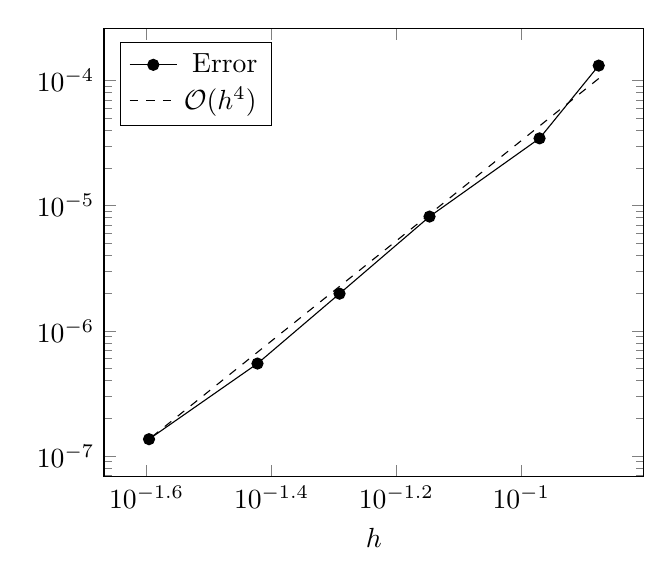
\begin{tikzpicture}
\begin{loglogaxis}[
    xlabel={$h$},
    legend pos=north west,
]

\addplot[black, mark=*] coordinates {(0.13307,0.000131393) (0.106989,3.44649e-05) (0.0713092,8.1769e-06) (0.0511671,1.98114e-06) (0.0378115,5.47747e-07) (0.0253431,1.36302e-07)};
\addlegendentry{$\LT$ Error}

\addplot[black, dashed] coordinates {(0.13307,0.0001036057614569891) (0.0253431,1.36302e-07)};
\addlegendentry{$\mathcal{O}(h^{4})$}

\end{loglogaxis}
\end{tikzpicture}
\end{subfigure}
\hfill
\begin{subfigure}[b]{0.45\textwidth}
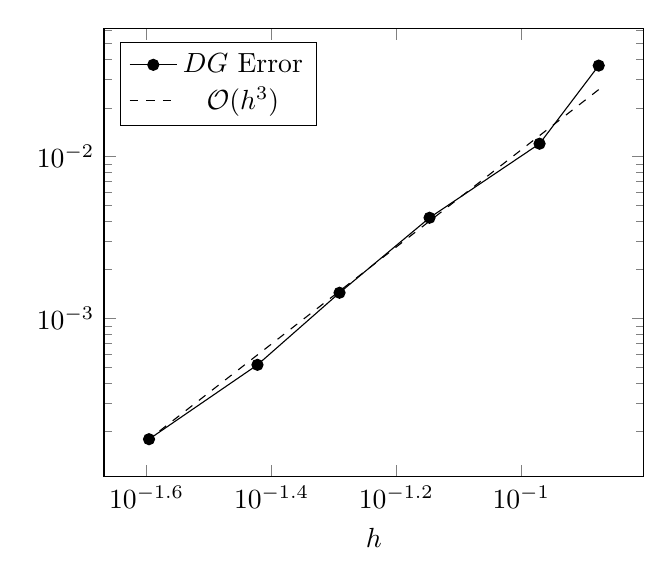
\begin{tikzpicture}
\begin{loglogaxis}[
    xlabel={$h$},
    legend pos=north west,
]

\addplot[black, mark=*] coordinates {(0.13307,0.036557) (0.106989,0.0120258) (0.0713092,0.00419264) (0.0511671,0.00144215) (0.0378115,0.000517054) (0.0253431,0.000179452)};
\addlegendentry{$DG$ Error}

\addplot[black, dashed] coordinates {(0.13307,0.025978230256595083) (0.0253431,0.000179452)};
\addlegendentry{$\mathcal{O}(h^{3})$}

\end{loglogaxis}
\end{tikzpicture}
\end{subfigure}
    \caption{$\LT$ and DG errors versus mesh size on a sequence of uniform meshes over a square domain. $k = 2$ (top), $k = 3$ (bottom) and $N \in \{125, 250, \dots, 4000\}$.}
\end{figure}

\newpage
\begin{figure}[!ht]
    % Errors v Size template for TikZ.

\begin{subfigure}[b]{0.45\textwidth}
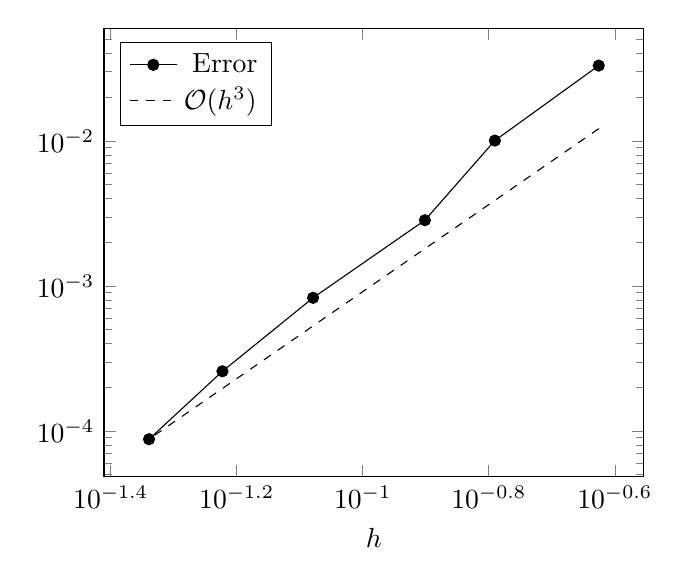
\begin{tikzpicture}
\begin{loglogaxis}[
    xlabel={$h$},
    legend pos=north west,
]

\addplot[black, mark=*] coordinates {(0.236846,0.033079) (0.162063,0.0100577) (0.125487,0.00284011) (0.0834066,0.000829064) (0.0598985,0.000258195) (0.0458041,8.78696e-05)};
\addlegendentry{$\LT$ Error}

\addplot[black, dashed] coordinates {(0.236846,0.012148530558035811) (0.0458041,8.78696e-05)};
\addlegendentry{$\mathcal{O}(h^{3})$}

\end{loglogaxis}
\end{tikzpicture}
\end{subfigure}
\hfill
\begin{subfigure}[b]{0.45\textwidth}
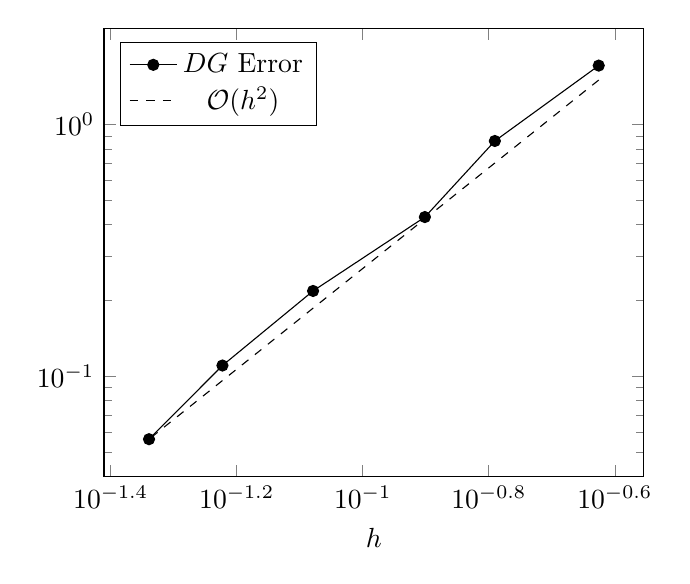
\begin{tikzpicture}
\begin{loglogaxis}[
    xlabel={$h$},
    legend pos=north west,
]

\addplot[black, mark=*] coordinates {(0.236846,1.71328) (0.162063,0.859474) (0.125487,0.428497) (0.0834066,0.217901) (0.0598985,0.110162) (0.0458041,0.0561394)};
\addlegendentry{$DG$ Error}

\addplot[black, dashed] coordinates {(0.236846,1.501036204482293) (0.0458041,0.0561394)};
\addlegendentry{$\mathcal{O}(h^{2})$}

\end{loglogaxis}
\end{tikzpicture}
\end{subfigure}
    % Errors v Size template for TikZ.

\begin{subfigure}[b]{0.45\textwidth}
\begin{tikzpicture}[scale=.6]
\begin{loglogaxis}[
    xlabel={$h$},
    legend pos=north west,
]

\addplot[solarized-base02, mark=*] coordinates {(0.236846,0.00236589) (0.162063,0.000476832) (0.125487,0.000110835) (0.0834066,2.72149e-05) (0.0598985,6.75002e-06) (0.0458041,1.74035e-06)};
\addlegendentry{$\LT$ Error}

\addplot[solarized-base02, dashed] coordinates {(0.236846,0.0012441805245544592) (0.0458041,1.74035e-06)};
\addlegendentry{$\mathcal{O}(h^{4})$}

\end{loglogaxis}
\end{tikzpicture}
\end{subfigure}
\hfill
\begin{subfigure}[b]{0.45\textwidth}
\begin{tikzpicture}[scale=.6]
\begin{loglogaxis}[
    xlabel={$h$},
    legend pos=north west,
]

\addplot[solarized-base02, mark=*] coordinates {(0.236846,0.354304) (0.162063,0.112679) (0.125487,0.0379581) (0.0834066,0.0128848) (0.0598985,0.00442298) (0.0458041,0.0015715)};
\addlegendentry{$DG$ Error}

\addplot[solarized-base02, dashed] coordinates {(0.236846,0.2172698609297559) (0.0458041,0.0015715)};
\addlegendentry{$\mathcal{O}(h^{3})$}

\end{loglogaxis}
\end{tikzpicture}
\end{subfigure}
    \caption{$\LT$ and DG errors versus mesh size on a sequence of uniform meshes over an L-shaped domain. $k = 2$ (top), $k = 3$ (bottom) and $N \in \{125, 250, \dots, 4000\}$.}
\end{figure}

\newpage
\subsection{Pathological solutions}

Tests over a sequence of uniform meshes, using pathological functions as exact solutions, highlight the need for an adaptive algorithm.

\cite{Antonietti2013} The pathological function for the square domain is:

\begin{gather} \label{pathological_square}
    u(x, y) = \frac{1 - e^{-100x}}{1 - e^{-100}} \sin(\pi y) (1 - x),
\end{gather}

which exhibits a strong boundary layer along the line $x = 0$.

For the L-shaped domain, the pathological function is:

\begin{gather} \label{pathological_lshape}
    u(\rho, \theta) = \rho^{2 / 3} \sin\left(\frac{2 \theta}{3}\right),
\end{gather}

for which $f = 0$ and $u$ is analytical in $\Omega \setminus \Vector{0}$, but $\grad{u}$ is singular at the origin.

Error trends in the following pages.

\newpage
\subsubsection{Errors}

Despite being a smooth function, the pathological solution over the square achieves the expected convergence rate, albeit at a slower pace.

\begin{figure}[!ht]
    % Errors v Size template for TikZ.

\begin{subfigure}[b]{0.45\textwidth}
\begin{tikzpicture}
\begin{loglogaxis}[
    xlabel={$h$},
    legend pos=north west,
]

\addplot[solarized-base02, mark=*] coordinates {(0.13307,0.0281162) (0.106989,0.0180826) (0.0713092,0.0115527) (0.0511671,0.00546711) (0.0378115,0.00254289) (0.0253431,0.00101081) (0.0205266,0.000422415)};
\addlegendentry{$\LT$ Error}

\addplot[solarized-base02, dashed] coordinates {(0.13307,0.11508765584587866) (0.0205266,0.000422415)};
\addlegendentry{$\mathcal{O}(h^{3})$}

\end{loglogaxis}
\end{tikzpicture}
\end{subfigure}
\hfill
\begin{subfigure}[b]{0.45\textwidth}
\begin{tikzpicture}
\begin{loglogaxis}[
    xlabel={$h$},
    legend pos=north west,
]

\addplot[solarized-base02, mark=*] coordinates {(0.13307,6.12566) (0.106989,5.25995) (0.0713092,4.30988) (0.0511671,2.91652) (0.0378115,1.85839) (0.0253431,1.02974) (0.0205266,0.5601)};
\addlegendentry{$DG$ Error}

\addplot[solarized-base02, dashed] coordinates {(0.13307,23.539208068455636) (0.0205266,0.5601)};
\addlegendentry{$\mathcal{O}(h^{2})$}

\end{loglogaxis}
\end{tikzpicture}
\end{subfigure}
    % Errors v Size template for TikZ.

\begin{subfigure}[b]{0.45\textwidth}
\begin{tikzpicture}[scale=.6]
\begin{loglogaxis}[
    xlabel={$h$},
    legend pos=north west,
]

\addplot[solarized-base02, mark=*] coordinates {(0.13307,0.0129373) (0.106989,0.00691892) (0.0713092,0.00333505) (0.0511671,0.0011295) (0.0378115,0.000395856) (0.0253431,0.000109201) (0.0205266,3.37306e-05)};
\addlegendentry{$\LT$ Error}

\addplot[solarized-base02, dashed] coordinates {(0.13307,0.05957672373397235) (0.0205266,3.37306e-05)};
\addlegendentry{$\mathcal{O}(h^{4})$}

\end{loglogaxis}
\end{tikzpicture}
\end{subfigure}
\hfill
\begin{subfigure}[b]{0.45\textwidth}
\begin{tikzpicture}[scale=.6]
\begin{loglogaxis}[
    xlabel={$h$},
    legend pos=north west,
]

\addplot[solarized-base02, mark=*] coordinates {(0.13307,5.22824) (0.106989,3.45593) (0.0713092,2.29411) (0.0511671,1.08811) (0.0378115,0.495229) (0.0253431,0.194102) (0.0205266,0.0764724)};
\addlegendentry{$DG$ Error}

\addplot[solarized-base02, dashed] coordinates {(0.13307,20.83503013128883) (0.0205266,0.0764724)};
\addlegendentry{$\mathcal{O}(h^{3})$}

\end{loglogaxis}
\end{tikzpicture}
\end{subfigure}
    \caption{$\LT$ and DG errors versus mesh size on a sequence of uniform meshes over a square domain. $k = 2$ (top), $k = 3$ (bottom) and $N \in \{125, 250, \dots, 8000\}$.}
\end{figure}

\newpage

Due to its nature, the pathological solution on the L-shaped domain does not reach the expected convergence rate.

\begin{figure}[!ht]
    % Errors v Size template for TikZ.

\begin{subfigure}[b]{0.45\textwidth}
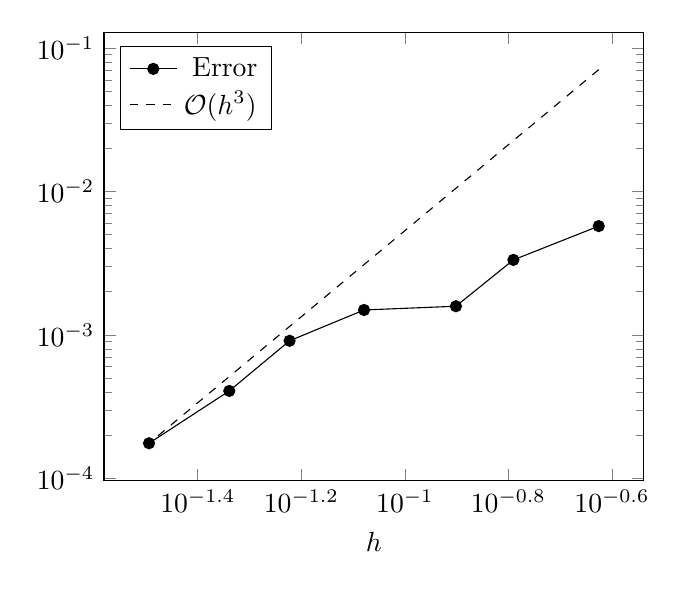
\begin{tikzpicture}
\begin{loglogaxis}[
    xlabel={$h$},
    legend pos=north west,
]

\addplot[black, mark=*] coordinates {(0.236846,0.00573887) (0.162063,0.00333593) (0.125487,0.00158497) (0.0834066,0.00149286) (0.0598985,0.000910291) (0.0458041,0.000406812) (0.0320544,0.000175592)};
\addlegendentry{$\LT$ Error}

\addplot[black, dashed] coordinates {(0.236846,0.07083370080315939) (0.0320544,0.000175592)};
\addlegendentry{$\mathcal{O}(h^{3})$}

\end{loglogaxis}
\end{tikzpicture}
\end{subfigure}
\hfill
\begin{subfigure}[b]{0.45\textwidth}
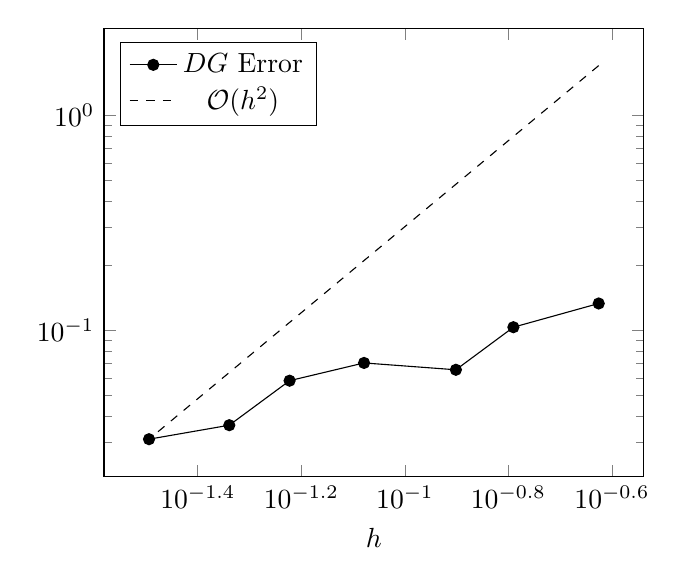
\begin{tikzpicture}
\begin{loglogaxis}[
    xlabel={$h$},
    legend pos=north west,
]

\addplot[black, mark=*] coordinates {(0.236846,0.13327) (0.162063,0.103364) (0.125487,0.0655286) (0.0834066,0.0705169) (0.0598985,0.0583046) (0.0458041,0.0362069) (0.0320544,0.0311668)};
\addlegendentry{$DG$ Error}

\addplot[black, dashed] coordinates {(0.236846,1.7015668612169044) (0.0320544,0.0311668)};
\addlegendentry{$\mathcal{O}(h^{2})$}

\end{loglogaxis}
\end{tikzpicture}
\end{subfigure}
    % Errors v Size template for TikZ.

\begin{subfigure}[b]{0.45\textwidth}
\begin{tikzpicture}
\begin{loglogaxis}[
    xlabel={$h$},
    legend pos=north west,
]

\addplot[solarized-base02, mark=*] coordinates {(0.236846,0.00261101) (0.162063,0.00162784) (0.125487,0.000513351) (0.0834066,0.000699775) (0.0598985,0.000454435) (0.0458041,0.000154545) (0.0320544,7.87786e-05)};
\addlegendentry{$\LT$ Error}

\addplot[solarized-base02, dashed] coordinates {(0.236846,0.23481285454935658) (0.0320544,7.87786e-05)};
\addlegendentry{$\mathcal{O}(h^{4})$}

\end{loglogaxis}
\end{tikzpicture}
\end{subfigure}
\hfill
\begin{subfigure}[b]{0.45\textwidth}
\begin{tikzpicture}
\begin{loglogaxis}[
    xlabel={$h$},
    legend pos=north west,
]

\addplot[solarized-base02, mark=*] coordinates {(0.236846,0.119546) (0.162063,0.0940845) (0.125487,0.0594576) (0.0834066,0.0630073) (0.0598985,0.0505441) (0.0458041,0.0336456) (0.0320544,0.0267768)};
\addlegendentry{$DG$ Error}

\addplot[solarized-base02, dashed] coordinates {(0.236846,10.801744041106874) (0.0320544,0.0267768)};
\addlegendentry{$\mathcal{O}(h^{3})$}

\addplot[solarized-base02, dotted] coordinates {(0.236846,0.10158063960750381) (0.0320544,0.0267768)};
\addlegendentry{$\mathcal{O}(h^{2/3})$}

\end{loglogaxis}
\end{tikzpicture}
\end{subfigure}
    \caption{$\LT$ and DG errors versus mesh size on a sequence of uniform meshes over an L-shaped domain. $k = 2$ (top), $k = 3$ (bottom) and $N \in \{125, 250, \dots, 8000\}$.}
\end{figure}